Multirotor er en samlebetegnelse på alle typer droner med 3 eller flere motorer. Den vanligste typen er quadcopter, altså en drone med fire armer og en motor på hver arm. Figur \ref{fig:dji-air-2} viser et populært quadcopter fra DJI.

\begin{figure}[htp]
    \centering
    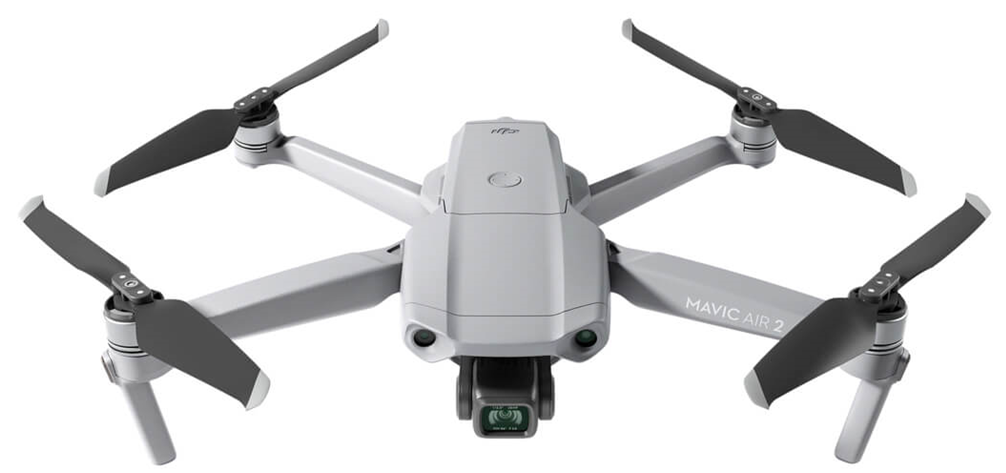
\includegraphics[width=0.7\columnwidth]{figures/dji-air-2}
    \caption{DJI Air 2}
    \label{fig:dji-air-2}
\end{figure}

\subsubsection{Komponenter}
Et quadcopter består i sin enkleste grad av en ramme, fire motorer, fire propeller, en flight controller, en mottaker og fire ESC ’er.
Flightcontrolleren er hjernen i drona. Denne består av en liten datamaskin, IMU og porter. Oppgaven til flightcontrolleren er å ta imot signaler fra sensorer og radiokontroller, og gi signal videre til ESC for å styre hastigheten til de individuelle motorene. 

\begin{figure}[htp]
    \centering
    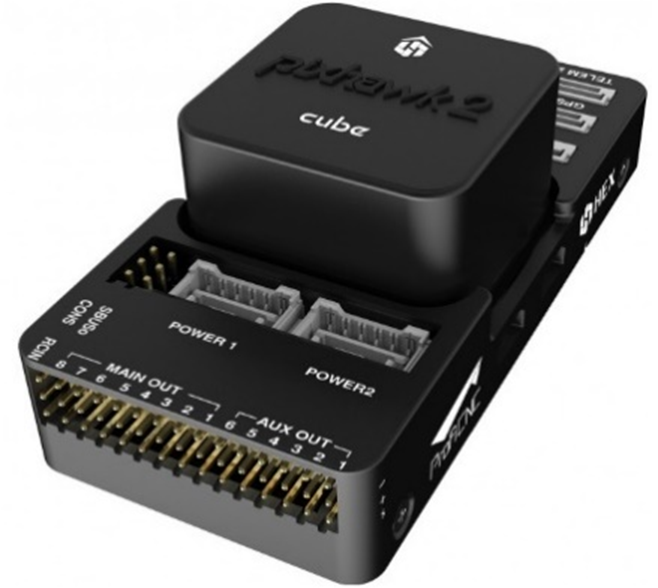
\includegraphics[width=0.4\columnwidth]{figures/pixhawk}
    \caption{Pixhawk Cube}
    \label{fig:pixhawk}
\end{figure}

Pixhawk, som vist i figur \ref{fig:pixhawk}, er en populær flightcontroller til utvikling av droner. Denne kan kjøre ardupilot programvare, som er opensource programvare laget for ROV, fly og multirotor. Grunnen til at pixhawk og ardupilot er så mye brukt er at det enkelt kan kobles på sensorer og utstyr, og man kan enkelt gjøre egne endringer i programvaren. 
En mottaker kobles til flightcontrolleren for at man skulle kunne gjennomføre manuell flygning og kunne bytte mellom ulike moduser under automatisk flyging med en radio. 
ESC (Electronic Speed Controller) er fartskontrolleren til motoren. Denne får signal fra flightcontrolleren om hvor fort motorene skal spinne, og gir deretter tilsvarende strøm til motorene. 

\begin{figure}[htp]
    \centering
    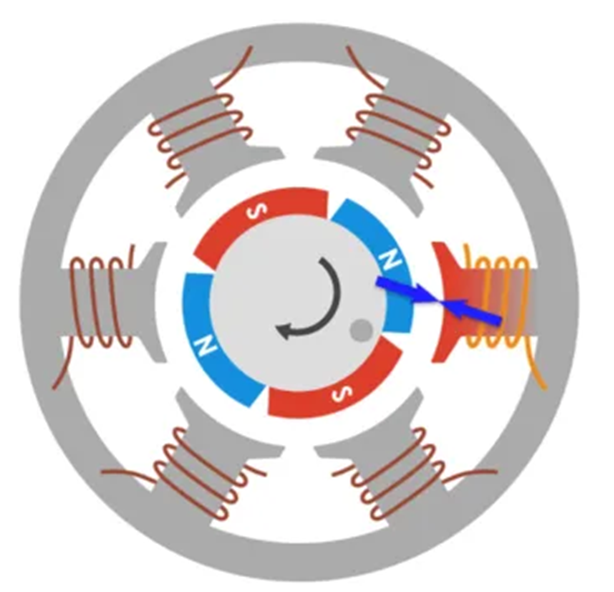
\includegraphics[width=0.4\columnwidth]{figures/dc-motor}
    \caption{Børsteløs DC-motor}
    \label{fig:dc-motor}
\end{figure}

Børsteløse DC motorer blir oftest brukt på quadcopter. Disse består av to deler. En stator og en rotor. Statoren er bygget opp av flere viklinger med kobbertråd. Rotoren er laget av en magnet. Når det blir satt strøm på ulike kobbertråd viklinger vil det skape et magnetfelt som får magneten i rotoren til å spinne i ønsket retning, som vist i Figur 21. På denne måten kan man enkelt øke og minke hastigheten på motoren.

\subsubsection{Styring}
En multirotor styres som tradisjonelle fly med pitch, yaw og roll. Illustrert i figur \ref{fig:akser}

\begin{figure}[htp]
    \centering
    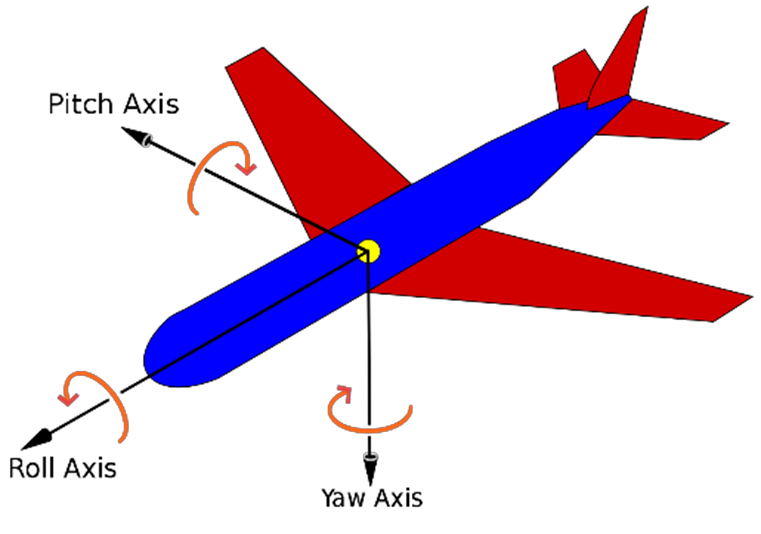
\includegraphics[width=0.4\columnwidth]{figures/akser}
    \caption{Akser på et luftfartøy}
    \label{fig:akser}
\end{figure}

For å rotere i de ulike aksene, må motorene spinne i ulike hastigheter.Figur \ref{fig:motor-rotasjon} viser det vanligste oppsettet for motorenes rotasjon:

\begin{itemize}
\item Pitch: for å få dronen til å bevege seg fremover må motor 3 og 4 spinne raskere enn motor 1 og 2.
\item Roll: For å få dronen til å bevege seg til venstre må motor 2 og 3 spinne raskere.
\item Yaw: For å dreie dronen mot høyre må motor 2 og 4 spinne fortere.
\end{itemize}

\begin{figure}[htp]
    \centering
    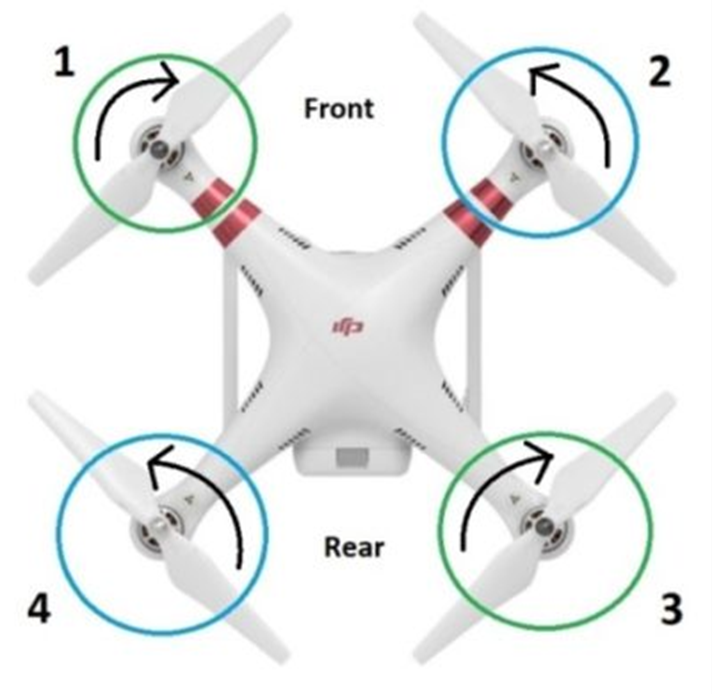
\includegraphics[width=0.4\columnwidth]{figures/motor-rotasjon}
    \caption{Rotasjonsretning på multirotor}
    \label{fig:motor-rotasjon}
\end{figure}

I tillegg til disse tre brukes throttle. Øking av throttle gjør at alle motorene spinner fortere, og dronen vil da få en akselerasjon normalt på planet til propellene. Altså rett opp dersom dronen står stille på bakken.
Dronen styres da ved å bruke pitch, roll og yaw for å oppnå ønsket rotasjon, og throttle for å skape en akselerasjon i ønsket retning. Illustrert i figur \ref{fig:krefter-pa-drone}. 

\begin{figure}[htp]
    \centering
    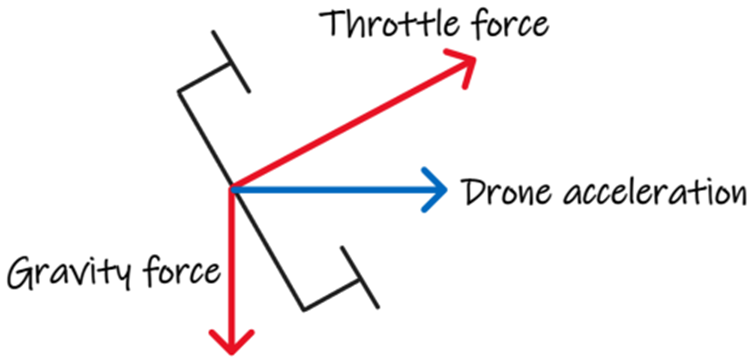
\includegraphics[width=0.5\columnwidth]{figures/krefter-pa-drone}
    \caption{Krefter i fartsretningen på en multirotor}
    \label{fig:krefter-pa-drone}
\end{figure}